% Set the Page Layout
\documentclass[12pt]{article}
\usepackage[inner = 2.0cm, outer = 2.0cm, top = 2.0cm, bottom = 2.0cm]{geometry}
\usepackage{biblatex}
\usepackage{graphicx}
% Package to write pseudo-codes
\usepackage{algorithm}

% Package for Hyperlinks
\usepackage[colorlinks = true, urlcolor = blue,  linkcolor = blue]{hyperref}

% Don't Remove the 'end' at the end of the algorithm
\usepackage{algpseudocode}

% Manually remove the 'end' for some sections
\algtext*{EndIf}
\algtext*{EndFor}
\algtext*{EndWhile}

% Define Left Justified Comments
\algnewcommand{\LeftComment}[1]{\Statex \(\triangleright\) #1}

% Remove the Numbering of the Algorithm
\usepackage{caption}
\DeclareCaptionLabelFormat{algnonumber}{Algorithm}
\captionsetup[algorithm]{labelformat = algnonumber}

% Define the command for a boldface instructions
\newcommand{\Is}{\textbf{ is }}
\newcommand{\To}{\textbf{ to }}
\newcommand{\Downto}{\textbf{ downto }}
\newcommand{\Or}{\textbf{ or }}
\newcommand{\And}{\textbf{ and }}
\newcommand{\NotEmpty}{\textbf{ not empty,}}
\newcommand{\Append}{\textbf{append}}
\newcommand{\Each}{\textbf{each }}
% Use them inside Math-Mode (Hence the space!)

\begin{titlepage}
   \begin{center}
       \vspace*{1cm}

       \textbf{Algorithmic-Pseudocode}

       \vspace{0.5cm}
        Thesis Subtitle
            
       \vspace{1.5cm}

       \textbf{Author Name}

       \vfill
            
       Algorithmic-Pseudocode
            
       \vspace{0.8cm}
     
       \includegraphics[width=0.4\textwidth]{university}
            
       title\\
       subtitle Name\\
       Date
            
   \end{center}
\end{titlepage}

\begin{document}

\begin{algorithm}

  \caption{Topological Sort using Kahn's algorithm  \cite{1}}
  
  \begin{algorithmic}[1]
        \Ensure The vertices are indexed from 1 to $V$
        \Require The Graph is a Directed Acyclic Graph
        
        \Statex
        
        \Function{$Topological\_Sort$}{$Adjacency\_List, Vertex\_Set$}
        
            \State $sorted \gets$ Empty List that will contain the Topological Ordering
            \State $queue \gets$ Empty queue to store elements with 0 in-degree
            \State $V \gets Vertex\_Set.\textbf{size}$
            
            \Statex 
            
            \For{$node = 1 \To V$}
                \State $in\_degree[node] \gets 0$ \Comment{Intialize in-degree}
            \EndFor
            
            \Statex
            
            \For{$node = 1 \To V$}
                \For{$\Each \textbf{child} \in adjacency[node]$}
                    \State $in\_degree[child] \gets in\_degree[child] + 1$ \Comment{Update in-degree}
                \EndFor
            \EndFor
            
            \Statex 
            
            \For{$node = 1 \To V$}
                \If{$in\_degree[node] \Is 0$}
                    \State $queue.push(node)$ \Comment {Collect the source vertices}
                \EndIf
            \EndFor
            
            \Statex
            
            \While {$queue \ is \NotEmpty$}
                \State $current \gets queue.front$
                \State $queue.pop$
                
                \State $sorted.\Append(current)$
                
                \For{$\Each \textbf{child} \in adjacency[current]$}
                    \State $in\_degree[child] \gets in\_degree[child] - 1$ \Comment{Delete the $current$ vertex virtually}
                    \If{$in\_degree[child] \Is 0$}
                        \State $queue.push(child)$ \Comment{Capture the new source vertex}
                    \EndIf
                \EndFor
            \EndWhile
            
            \Statex
            
            
            \If{$sorted.\textbf{size} \neq Vertex\_Set.\textbf{size}$ }
                \State \Return \textbf{Error} \Comment{Graph has atleast one cycle}
            \Else
            \State \Return $sorted$
            \EndIf
            
            \Statex
            
        \EndFunction
  \end{algorithmic}
 
\end{algorithm}

\pagebreak

Example:
\begin{figure}[H]
\centering
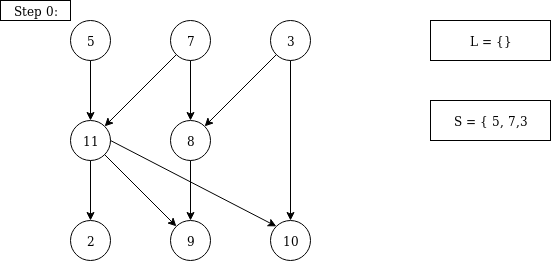
\includegraphics[width=100mm]{KahnAlgoStep1.png}
\caption{init state}
\end{figure}

\begin{figure}[H]
\centering
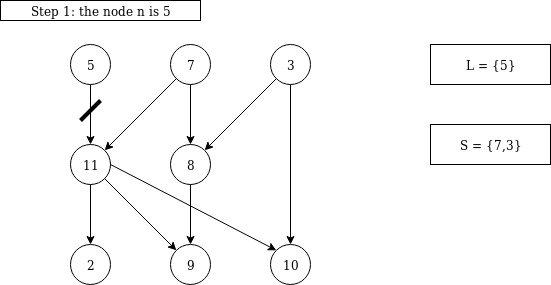
\includegraphics[width=100mm]{KahnAlgoStep2.png}
\caption{state 1}
\end{figure}

\begin{figure}[H]
\centering
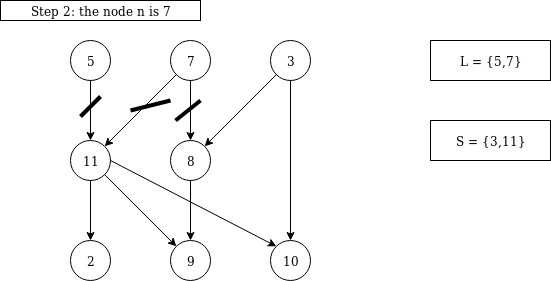
\includegraphics[width=100mm]{KahnAlgoStep3.png}
\caption{state 2}
\end{figure}

\begin{figure}[H]
\centering
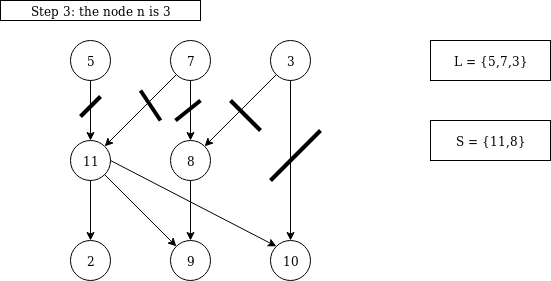
\includegraphics[width=100mm]{KahnAlgoStep4.png}
\caption{state 3}
\end{figure}
    
    
    \begin{figure}[H]
\centering
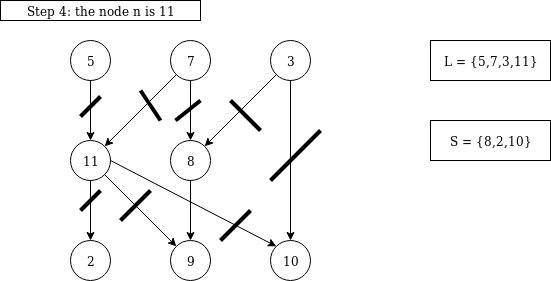
\includegraphics[width=100mm]{KahnAlgoStep5.png}
\caption{state 4 }
\end{figure}

\begin{figure}[H]
\centering
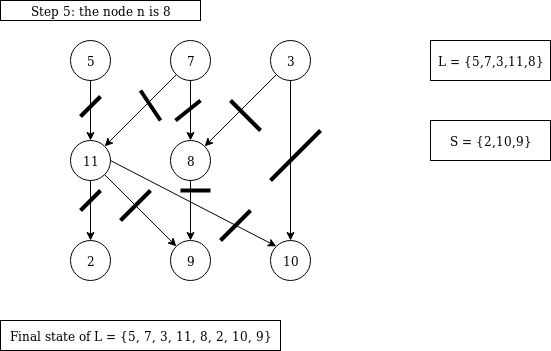
\includegraphics[width=100mm]{KahnAlgoStep6.png}
\caption{state 5}
\end{figure}

\begin{thebibliography}{1}
\bibitem{wikipedia} 
Topological sort: Kahn's algorithm \\ 
\href{https://en.wikipedia.org/wiki/Topological\_sorting\#Kahn's\_algorithm}{Link}
\end{thebibliography}



\end{document}
